% Drawing 147/07-3 -- folder 147, batch 07, archive page 140 (PDF page 141).
% Transcription: un arc de bande hachurée en forme de U, non recoupé, avec une flèche marquée $D'$ désignant l'âme de la bande.
% Kind: U-shaped hatched band with its core. Method 2 (schematic redraw from the facsimile). Status: ok.
% Notes: An arc of hatched band in the shape of a U, not crossing itself, with an arrow marked D' pointing to the core of the band (the core drawn as the middle line).
% Coordinates: 1 unit = 1 mm = 1/100 of the crop width (bbox in page fractions: [0.366, 0.416, 0.85, 0.564]).
% Redrawn by Claude (claude-opus-5-5), issue #73, 2026-11-07; not checked by a human; not compiled (no TeX in the session).
% Rights: reproduces part of the work -- behind RENDER_TRANSCRIPTS, never published by itself.
\documentclass[tikz,border=3pt]{standalone}
\usepackage{amsmath,amssymb}
\usetikzlibrary{patterns,arrows.meta}
\tikzset{pencil/.style={black!45}, struck/.style={black!35}, mark/.style={circle,draw,inner sep=1.3pt}, pt/.style={circle,fill,inner sep=0.9pt}, opt/.style={circle,draw,fill=white,inner sep=1.1pt}}
\begin{document}
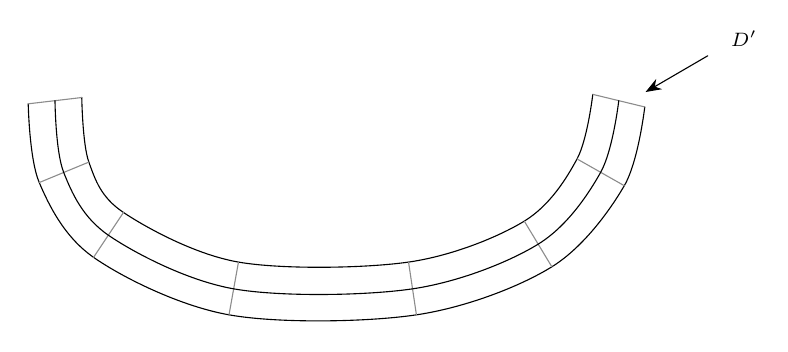
\begin{tikzpicture}[x=1mm,y=1mm,line cap=round,line join=round,font=\scriptsize]
\draw plot[smooth, tension=0.55] coordinates {(5.7,-12.9) (7.1,-22.9) (14,-32.4) (31.2,-39.7) (55,-39.7) (72.2,-33.6) (81.4,-23.3) (84,-13.3)};
\draw plot[smooth, tension=0.55] coordinates {(12.5,-12.1) (13.4,-20.3) (17.8,-26.7) (32.4,-33) (54,-33) (68.7,-27.8) (75.4,-19.9) (77.4,-11.7)};
\draw[pencil] (5.7,-12.9) -- (12.5,-12.1);
\draw[pencil] (7.1,-22.9) -- (13.4,-20.3);
\draw[pencil] (14,-32.4) -- (17.8,-26.7);
\draw[pencil] (31.2,-39.7) -- (32.4,-33);
\draw[pencil] (55,-39.7) -- (54,-33);
\draw[pencil] (72.2,-33.6) -- (68.7,-27.8);
\draw[pencil] (81.4,-23.3) -- (75.4,-19.9);
\draw[pencil] (84,-13.3) -- (77.4,-11.7);
\draw plot[smooth, tension=0.55] coordinates {(9.1,-12.5) (10.2,-21.6) (15.9,-29.6) (31.8,-36.4) (54.5,-36.4) (70.5,-30.7) (78.4,-21.6) (80.7,-12.5)};
\draw[-{Stealth[length=2mm]}] (92,-6.8) -- (84.1,-11.4);
\node[inner sep=1pt] at (96.6,-4.6) {\scriptsize $D'$};
\end{tikzpicture}
\end{document}
